% XeLaTeX can use any Mac OS X font. See the setromanfont command below.
% Input to XeLaTeX is full Unicode, so Unicode characters can be typed directly into the source.

% The next lines tell TeXShop to typeset with xelatex, and to open and save the source with Unicode encoding.

%!TEX TS-program = xelatex
%!TEX encoding = UTF-8 Unicode

\documentclass[11pt]{article}


%%%%%%%%%%%%%%%
\def\Type{ApplicationDJ}
\def\TypeNum{Markov Chains: KEY}
\def\TypeTitle{}
\def\Semester{Spring 205}
\def\Course{Math 1190/1210}
\def\Targets{{\bf\color{Goldenrod}AD1}}

\usepackage{preambleDJ}
%\usepackage{kbordermatrix}
\newcommand{\fs}[1]{$\mbox{\footnotesize #1}$}
\usetikzlibrary{arrows}

\begin{document}
\pagestyle{otherpages}
\thispagestyle{firstpage}
\vspace*{.35in}
\mpageT{.6}{.4}{
A Markov Chain is a mathematical object first described by Andrei Markov in $1906$.  It  describes  the probability of transitioning from one state to another with the important assumption that this transition is independent of the starting state. The notation that we will use for this is $$P(E_2|E_1)$$ which means {\em ``The probability of moving from state $E_1$ to $E_2$ (in one step)."}
~\\\\
Markov initially used this idea to study the distribution of vowels in Alexander Pushkin's novel {\em Eugene Onegin}. Today, Markov Chains have applications in health, business, finance, Google's Page Rank algorithm, detecting gerrymandering, and in many other fields.  
}{
\graphicsR{aaMarkov}{1.75} 
}~\\ \vs{.1} \\
The following game is an example of a Markov Chain.
\quot{
A player starts with $\$80$. A player bets $\$40$ each time a coin is flipped. If the result is Heads, the player receives original bet back and an additional $\$40$. Tails means player loses the original bet. The coin is flipped twice.
}  
The transition  diagram below  captures the possible states after each coin flip.
	\begin{center}
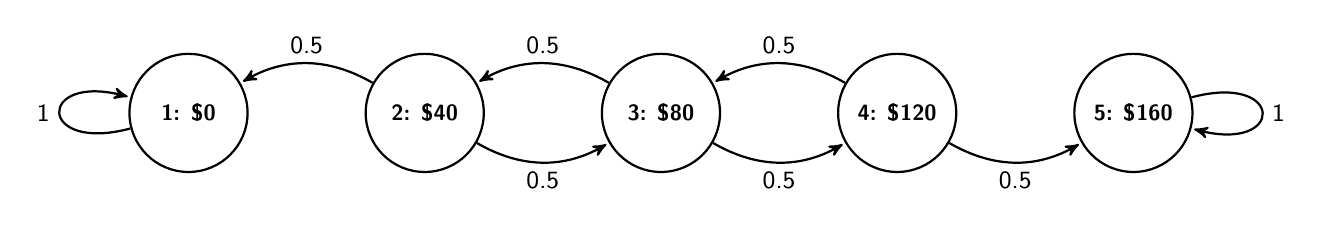
\begin{tikzpicture}[->,>=stealth',shorten >=1pt,auto,node distance=3cm,
                    thick,main node/.style={circle,draw,minimum size=1.5cm,font=\sffamily\footnotesize\bfseries}]

%  \node[main node] (1) [ left of=1] {1: \$0};
%  \node[main node] (2) {2: \$40};
% \node[main node] (3) [ right of=2] {3: \$80};
%  \node[main node] (4) [below right of=1] {4};

  \node[main node] (1)  {1: \$0};
    \node[main node] (2) [ right of=1] {2: \$40};
  \node[main node] (3) [ right of=2] {3: \$80};
    \node[main node] (4) [  right of=3] {4: \$120};
 \node[main node] (5) [ right of=4] {5: \$160};

  \path[every node/.style={font=\sffamily\small}]
    (1)     %edge [bend right] node  {0.4} (1)
   %     edge node {0.3} (4)
        edge [loop left] node {1} (1)
(2)        edge [bend right] node[above] {0.5} (1)  
                edge [bend right] node[below] {0.5} (3)

(3)        edge [bend right] node[above] {0.5} (2)  
                edge [bend right] node[below] {0.5} (4)
(4)        edge [bend right] node[above] {0.5} (3)  
                edge [bend right] node[below] {0.5} (5)
    (5)     %edge node [bend left] {0.2} (2)
       edge [loop right] node {1} (5);
 %   (4) edge node [left] {0.2} (3)
   %     edge [loop right] node {0.6} (4)
     %   edge [bend right] node[right] {0.2} (1);
\end{tikzpicture}
\end{center}
\itemI{
\item Note that the probability of moving from state $3$ ($E_3=\$80$) to state $4$ ( $E_4=\$120$) is $0.5=50\%$.  Using our new mathematical language, we can also say $\ds P(E_4|E_3)=0.5$.
\item We have assumed only two coin flips, so if we reach $E_1=\$0$ in exactly two coin flips, we will stay there with $100\%$ probability because there will be no more coin flips.  
\item Using probability notation: $P(E_1|E_1)=1$. Similarly $P(E_5|E_5)=1$
}
A {\em transition matrix} $P$ captures this same information for each of our $5$ possible states.\\
\mpageT{.3}{.7}[\hs{.1}]{
\large{	
$$P=
 \begin{blockarray}{cccccc}
&\fs{1}& \fs{2} &\fs{3} &\fs{4}&\fs{5}   \\
 \begin{block}{c[ccccc]}
\fs{1} & 1& 0.5 & 0 &0&0 \\
 \fs{2} & 0&0 &0.5&0&0 \\
 \fs{3}& 0&0.5&0&0.5&0\\
\fs{4} & 0& 0 & 0.5 &0&0 \\
\fs{5} & 0& 0 & 0 &0.5&1 \\
 \end{block}
 \end{blockarray}
$$
}
}{
\itemI{
\item Notation: We denote each member of the matrix by $P_{\text{row, column}}$.  $P_{1,2}=0.5$ is the element on the first row and $2nd$ column.
\item Interpretation: $P_{\text{row, column}}=P(E_{\text{row}}|E_{\text{column}})$ so $P_{2,3}=0.5=P(E_2|E_3)$ is the probability that the player will have $\$40$ (i.e. state $2$) after starting with $\$80$ (state $3$) after flipping the coin once. 
\item Each column sums up to $1$. This reflects the reality that when starting in state $i$, the probability that we move to one of states $1$ through $5$ must sum to be $1$.
}
}
\newpage

\mpageT{.7}{.3}[\hs{.1}]{
The  {\em transition matrix} $P$ is reproduced here for your convenience.\\\\
A {\em state vector} represents the probability we will be in one of our $5$ states. For example, we start the game with $\$80$ which means we have $100\%$ probability that we are in state $\# 3$ and $0\%$ probability we are in the other states. }{
\large{	
$$P=
 \begin{blockarray}{cccccc}
&\fs{1}& \fs{2} &\fs{3} &\fs{4}&\fs{5}   \\
 \begin{block}{c[ccccc]}
\fs{1} & 1& 0.5 & 0 &0&0 \\
 \fs{2} & 0&0 &0.5&0&0 \\
 \fs{3}& 0&0.5&0&0.5&0\\
\fs{4} & 0& 0 & 0.5 &0&0 \\
\fs{5} & 0& 0 & 0 &0.5&1 \\
 \end{block}
 \end{blockarray}
$$
}
}\vs{.1} ~\\ 
We capture this information in vector $S$.
\large{	
$$S=
 \begin{blockarray}{cc}
 \begin{block}{c[c]}
\fs{1} & 0 \\
 \fs{2} & 0 \\
 \fs{3}& 1\\
\fs{4} & 0 \\
\fs{5} & 0 \\
 \end{block}
 \end{blockarray}
$$
}


\mpageT{.7}{.3}{The power of using matrix/vector notation is that we can represent a coin flip by matrix-vector multiplication.  For example, the state vector after one coin flip show that when we start with $\$ 80$, there is a $50\%$ probability we will be in state $2$ (i.e. $\$40$) and a $50\%$ probability we will be in state $4$ (i.e. $\$120$) 
}{
\large{	
$$S_1=P\cdot S=
 \begin{blockarray}{cc}
 \begin{block}{c[c]}
\fs{1} & 0 \\
 \fs{2} & 0.5 \\
 \fs{3}& 0\\
\fs{4} & 0.5 \\
\fs{5} & 0 \\
 \end{block}
 \end{blockarray}
$$
}
}
\enum{
\item Find the probability distribution for all $5$ states after $2$ coin flips.  That is, find $$S_2=P\cdot S_1=P\cdot (P\cdot S)=P^2\cdot S.$$
\mpageT{.6}{.4}[\hs{.1}]{
\itemI{
\item Go to \href{https://www.desmos.com/matrix}{desmos.com/matrix}
\item Type in``$P=$" and click {\em New Matrix}. Choose $5$ rows and $5$ columns and create matrix $P$.
\item Type in ``$S=$" and click {\em New Matrix}. Choose $5$ rows and $1$ column and create vector $S$.
\item Type in ``$P^2\cdot S$" to see resulting state vector $S_2$. Use this to create a histogram representing probability the player will be in each of the $5$ states.
}
}{
%\graphicsR{histogram160Bars}{2.5}	
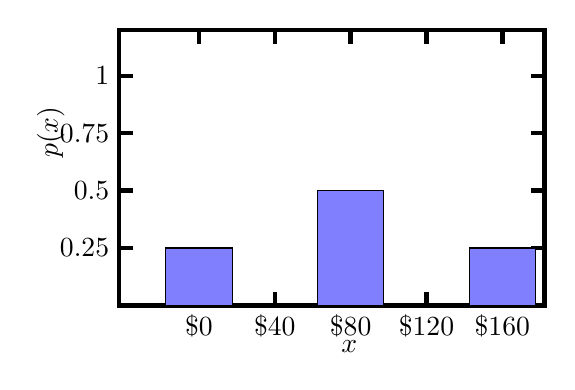
\begin{tikzpicture}
\begin{axis}[
	x label style={anchor=west},
xlabel={$x$},
xtick       = {1,2,3,4,5},
xticklabels = {$\$0$,$\$40$,$\$80$,$\$120$,$\$160$},
xticklabel style={anchor=north},
y label style={anchor=west},
ylabel={$p(x)$},
ytick={0.25,0.5,0.75,1},
%yticklabels = {$c$},
enlarge x limits={.01}, % Adjusts spacing between bars and axis limits
samples     = 320,
%domain      = -2.5:2.5,
%restrict y to domain=-6.5:6.5,
xmin =0, xmax = 5.5,
ymin = 0, ymax = 1.2,
axis line style = { ultra thick, -},
every major tick/.append style={ultra thick, black, major tick length=5pt},
width=2.75in, height=2in
%  grid=both, grid style=solid
]
\addplot[ybar, bar shift=0,   bar width=24pt,  fill=blue!50] plot coordinates {
(1,.25)  (2,0) (3,0.5) (4,0) (5,0.25) 
};
\end{axis}
\end{tikzpicture}
}

\newpage
\item {\em Game Scenario $\#2$}. A player starts with \$120 and bet  $\$40$ each time a coin is flipped. Heads means the player receives original bet back and an additional $\$40$.  Tails means the player loses $40$. The player has decided that they will stop  stops either when they run out of money or when they reach $\$200$. The following transition diagram represents this scenaro.
\begin{center}
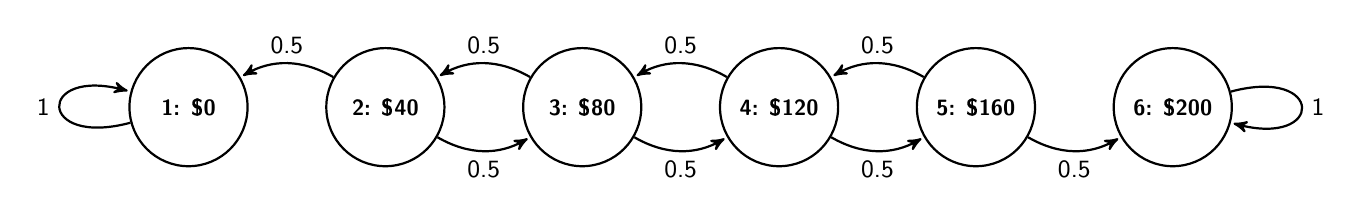
\begin{tikzpicture}[->,>=stealth',shorten >=1pt,auto,node distance=2.5cm,
                    thick,main node/.style={circle,draw,minimum size=1.5cm,font=\sffamily\footnotesize\bfseries}]

  \node[main node] (1)  {1: \$0};
    \node[main node] (2) [ right of=1] {2: \$40};
  \node[main node] (3) [ right of=2] {3: \$80};
    \node[main node] (4) [  right of=3] {4: \$120};
 \node[main node] (5) [ right of=4] {5: \$160};
  \node[main node] (6) [ right of=5] {6: \$200};

  \path[every node/.style={font=\sffamily\small}]
    (1)     %edge [bend right] node  {0.4} (1)
   %     edge node {0.3} (4)
        edge [loop left] node {1} (1)
(2)        edge [bend right] node[above] {0.5} (1)  
                edge [bend right] node[below] {0.5} (3)

(3)        edge [bend right] node[above] {0.5} (2)  
                edge [bend right] node[below] {0.5} (4)
(4)        edge [bend right] node[above] {0.5} (3)  
                edge [bend right] node[below] {0.5} (5)
(5)        edge [bend right] node[above] {0.5} (4)  
                edge [bend right] node[below] {0.5} (6)
    (6)     %edge node [bend left] {0.2} (2)
       edge [loop right] node {1} (6);
 %   (4) edge node [left] {0.2} (3)
   %     edge [loop right] node {0.6} (4)
     %   edge [bend right] node[right] {0.2} (1);
\end{tikzpicture}
\end{center}

\tasksA{2}{
\task Create transition matrix $P$ that represents this transition diagram. Consider how many states you have in order to determine how many columns and rows are needed.
\sol{
\large{	
$$P=
 \begin{blockarray}{ccccccc}
&\fs{1}& \fs{2} &\fs{3} &\fs{4}&\fs{5}  &\fs{6}   \\
 \begin{block}{c[cccccc]}
\fs{1} & 1& 0.5 & 0 &0&0&0 \\
 \fs{2} & 0&0 &0.5&0&0 &0\\
 \fs{3}& 0&0.5&0&0.5&0&0\\
\fs{4} & 0& 0 & 0.5 &0&0.5 &0\\
\fs{5} & 0& 0 & 0 &0.5&0&0 \\
\fs{6} &0 & 0& 0 & 0 &0.5&1 \\
 \end{block}
 \end{blockarray}
$$
}

}

\task Create the state vector $S$ that represents starting with $\$120$. 
\sol{
\large{	
$$S=
 \begin{blockarray}{cc}
 \begin{block}{c[c]}
\fs{1} & 0 \\
 \fs{2} & 0 \\
 \fs{3}& 0\\
\fs{4} & 1 \\
\fs{5} & 0 \\
\fs{6} & 0 \\
 \end{block}
 \end{blockarray}
$$
}
}
\task Go to \href{https://www.desmos.com/matrix}{desmos.com/matrix} and update the size of $P$ and $S$ for this new scenario.  Find the state vector after $3$ coin flips and use this to create a histogram representing the probability to be in each state.  {\em Hint:} $S_3=P\cdot S_2=\cdots ?$
%\graphicsL{histogram200Bars}{2.75}
\begin{flushleft}
\hs{-1}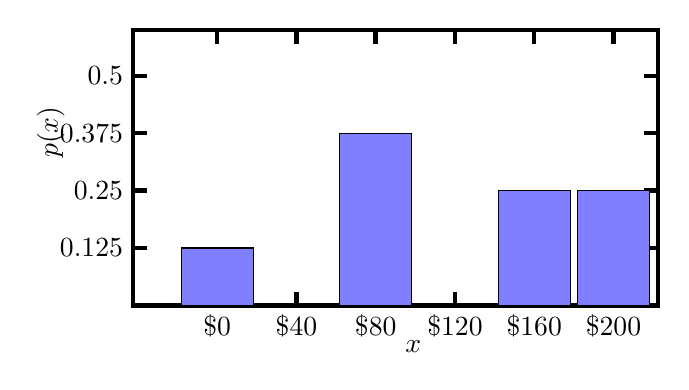
\begin{tikzpicture}
\begin{axis}[
	x label style={anchor=west},
xlabel={$x$},
xtick       = {1,2,3,4,5,6},
xticklabels = {$\$0$,$\$40$,$\$80$,$\$120$,$\$160$, $\$200$},
xticklabel style={anchor=north},
y label style={anchor=west},
ylabel={$p(x)$},
ytick={0.125,0.25,0.375,0.5},
yticklabels = {$0.125$,$0.25$, $0.375$, $0.5$},
enlarge x limits={.01}, % Adjusts spacing between bars and axis limits
samples     = 320,
%domain      = -2.5:2.5,
%restrict y to domain=-6.5:6.5,
xmin =0, xmax = 6.5,
ymin = 0, ymax = 0.6,
axis line style = { ultra thick, -},
every major tick/.append style={ultra thick, black, major tick length=5pt},
width=3.25in, height=2in
%  grid=both, grid style=solid
]
\addplot[ybar, bar shift=0,   bar width=26pt,  fill=blue!50] plot coordinates { (1,0.125)  (2,0) (3,0.375) (4,0) (5,0.25) (6,0.25) };
\end{axis}
\end{tikzpicture}
\end{flushleft}
\task What's the probability that the player will leave the game with $\$200$? $\$0$? {\em Hint:} How many coin flips will be needed to find this and how to use Desmos to estimate these probabilities.
\sol{While it's possible to reach $200$ in two coin flips, it could take many, many, many more to reach $\$ 200$.  In other words we need to find $$ \ds \limn S_n=\limn P^n\cdot S.$$ Since this is not possible in Desmos, and the techniques to do this outside of Desmos are outside of the scope of this course, we will estimate with larger and larger values for $n$ until the values for $S_n$ stabilize. For example when $n=30,000$,
\large{	
$$S_{30,000}=P^{30,000}\cdot S=
 \begin{blockarray}{cc}
 \begin{block}{c[c]}
\fs{1} & 0.4 \\
 \fs{2} & 0 \\
 \fs{3}& 0\\
\fs{4} & 0 \\
\fs{5} & 0 \\
\fs{6} & 0.6 \\
 \end{block}
 \end{blockarray}
$$
}
When the player starts with $\$120$, there is a $40\%$ chance to have $\$0$ and $60\%$ chance to have $\$200$ at the end of the game play.
}
\task Let's assume we start with $\$80$ instead of $\$120$. What's the probability the player will leave the game with $\$200$? Update the state vector $S$ and use Desmos to estimate this probability. 
\sol{The original state vectors becomes
\large{	
$$S=
 \begin{blockarray}{cc}
 \begin{block}{c[c]}
\fs{1} & 0 \\
 \fs{2} & 0 \\
 \fs{3}& 1\\
\fs{4} & 0 \\
\fs{5} & 0 \\
\fs{6} & 0 \\
 \end{block}
 \end{blockarray}
$$
}
We again need to to find $$ \ds \limn S_n=\limn P^n\cdot S.$$ We estimate with \ larger and larger values for $n$ until the values for $S_n$ stabilize. For example when $n=30,000$,
\large{	
$$S_{30,000}=P^{30,000}\cdot S=
 \begin{blockarray}{cc}
 \begin{block}{c[c]}
\fs{1} & 0.6 \\
 \fs{2} & 0 \\
 \fs{3}& 0\\
\fs{4} & 1 \\
\fs{5} & 0 \\
\fs{6} & 0.4 \\
 \end{block}
 \end{blockarray}
$$
}
When the player starts with $\$80$, there is $60\%$ chance to have $\$0$ and $40\%$ chance to have $\$200$ when game play ends.
}

\task  Let's assume we start with $\$160$ instead of $\$120$. What's the probability the player will leave the game with $\$200$? Update the state vector $S$ and use Desmos to estimate this probability. 
\sol{The original state vectors becomes
\large{	
$$S=
 \begin{blockarray}{cc}
 \begin{block}{c[c]}
\fs{1} & 0 \\
 \fs{2} & 0 \\
 \fs{3}& 0\\
\fs{4} & 0 \\
\fs{5} & 1 \\
\fs{6} & 0 \\
 \end{block}
 \end{blockarray}
$$
}

We again need to to find $$ \ds \limn S_n=\limn P^n\cdot S.$$ We estimate with \ larger and larger values for $n$ until the values for $S_n$ stabilize. For example when $n=30,000$,
\large{	
$$S_{30,000}=P^{30,000}\cdot S=
 \begin{blockarray}{cc}
 \begin{block}{c[c]}
\fs{1} & 0.2 \\
 \fs{2} & 0 \\
 \fs{3}& 0\\
\fs{4} & 1 \\
\fs{5} & 0 \\
\fs{6} & 0.8 \\
 \end{block}
 \end{blockarray}
$$
}
When the player starts with $\$160$ there is a $20\%$ chance to have $\$0$ and $80\%$ chance to have $\$200$.
}

}
\newpage
\item  {\em Modeling Spread of a Disease}  Let us consider how we might use a Markov Chain to model the spread of a disease. We assume that the population is divided into $3$ categories:   State $1$, Susceptible (S), State $2$,  Infected (I) or  State $3$, Recovered (R).  The fraction of the population in each category after $n$ weeks is $S_n$, $I_n$ and $R_n$. Note that $S_n+I_n+R_n=N$ where $N$ represents the total population.  The transition diagram below represents the portion of the population that transitions from one category to another each week.
\begin{center}
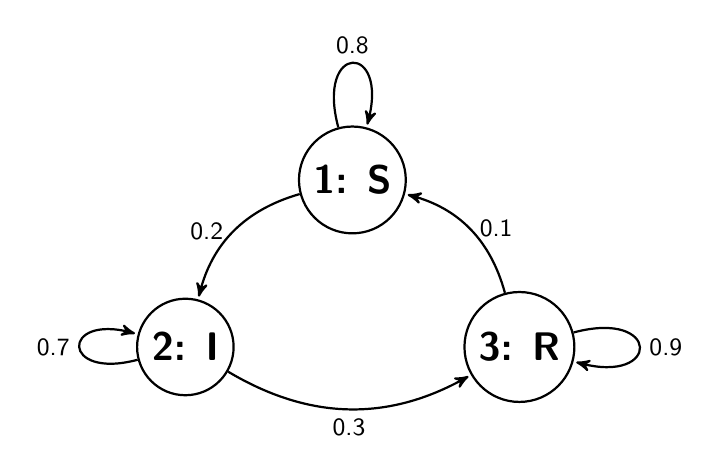
\begin{tikzpicture}[->,>=stealth',shorten >=1pt,auto,node distance=3cm,
                    thick,main node/.style={circle,draw,font=\sffamily\Large\bfseries}]

  \node[main node] (1) {1: S};
  \node[main node] (2) [below left of=1] {2: I};
  \node[main node] (3) [below right of=1] {3: R};
%  \node[main node] (4) [below right of=1] {4};

  \path[every node/.style={font=\sffamily\small}]
    (1)  edge [bend right] node[left] {0.2} (2)
        edge [loop above] node {0.8} (1)
%                edge [bend left] node {0.3} (3)
    (2) 
    %edge [bend right] node  {0.4} (1)
   %     edge node {0.3} (4)
        edge [loop left] node {0.7} (2)
        edge [bend right] node[below] {0.3} (3)
    (3) %edge node [bend left] {0.2} (2)
       edge [bend right] node[right] {0.1} (1)
       edge [loop right] node {0.9} (3);
 %   (4) edge node [left] {0.2} (3)
   %     edge [loop right] node {0.6} (4)
     %   edge [bend right] node[right] {0.2} (1);
\end{tikzpicture}
\end{center}
\tasksA{2}{
\task Create the transition matrix associated with the transition diagram here and in Desmos.\\
\sol{
\large{	
$$P=
 \begin{blockarray}{cccc}
&\fs{1}& \fs{2} &\fs{3}    \\
 \begin{block}{c[ccc]}
\fs{1} & 0.8& 0 & 0.1  \\
 \fs{2} & 0.2&0.7 &0 \\
\fs{3} & 0& 0.3 & 0.9  \\
 \end{block}
 \end{blockarray}
$$
}
}

\task Let's assume that at the beginning of our model $95\%$ of the population is Susceptible, $4\%$ are Infected and $1\%$ have recovered. Find the initial state vector, Since we are already using $S$ to represent the Susceptible part of the population, we'll use $V$ for our state vector.  \\
\sol{
\large{	
$$V=
 \begin{blockarray}{cc}
 \begin{block}{c[c]}
\fs{1} & 0.95 \\
 \fs{2} & 0.04 \\
 \fs{3}& 0.01\\
 \end{block}
 \end{blockarray}
$$
}
}
\task After one week, what percentage of the population is Susceptible? Infected?\\ Recovered?
\sol{
\large{	
$$V_1=P\cdot V=
 \begin{blockarray}{cc}
 \begin{block}{c[c]}
\fs{1} & 0.761 \\
 \fs{2} & 0.218 \\
 \fs{3}& 0.021\\
 \end{block}
 \end{blockarray}
$$
}
}
\task After $10$ weeks, what percentage of the population is Susceptible? Infected? \\Recovered?
\sol{
\large{	
$$V_{10}=P^{10} \cdot V=
 \begin{blockarray}{cc}
 \begin{block}{c[c]}
\fs{1} & 0.266297 \\
 \fs{2} & 0.213964 \\
 \fs{3}& 0.519739\\
 \end{block}
 \end{blockarray}
$$
}
}
\task* After a long, long time, does this model predict that the disease will die out? Will everyone get the disease? Will there always be a portion of the population that is infected?
\sol{We want to find 
\al{
\limn V_{n}=\limn P^{n} \cdot V
}
This is difficult to find, so we estimate by using 
\al{
V_{1000}&= P^{1000}\cdot V\\
&= \begin{blockarray}{cc}
 \begin{block}{c[c]}
\fs{1} & 0.272727 \\
 \fs{2} & 0.181818 \\
 \fs{3}& 0.545454\\
 \end{block}
 \end{blockarray}
 }
This model predicts after a long time,
\itemI{
\item  $I \approx 18.18\%$ of the population will be infected. Thus the disease will not die out. 
\item  $S\approx 27.27\%$ of the population will still be susceptible. But since there is a $10\%$ chance that someone could move from Recovered to Susceptible, this does not address how many of the Susceptible will have never been infected or not. 
}
~\\\\
{\em Additional Observations} Using tools beyond the scope of this course, it is possible to find the infinite limit exactly.  It turns out that 
\large{	
$$T=\limn V_{n}=
 \begin{blockarray}{c}
 \begin{block}{[c]}
3/11 \\
 2/11 \\
 6/11\\
 \end{block}
 \end{blockarray}
 \approx 
  \begin{blockarray}{c}
  \begin{block}{[c]}
0.272727 \\
 0.181818 \\
 0.545454\\
 \end{block}
 \end{blockarray}
$$
}

$T$ is called the {\em steady state vector} and  has the property that $$P\cdot T=T$$

An alternative name for $T$ is the {\em eigenvector} with {\em eigenvalue} of $\lambda = 1$.
}
}

\newpage
\item  {\em The Structure of Focus} (Optional, Extra, if time). The attention span of a student is measured once every  minute during class.  There are $4$ distinct States of Attention that the student cycles through.  The states are
\enumRo{
\item {\em Flow} (F): Deep, high-performance concentration. Time passes quickly; learning is maximized.
\item {\em Neutral} (N): Standard "listening" mode. The student is paying attention but is easily swayed.
\item {\em Distracted} (D): Attention has shifted to external stimuli (whispers, phone notifications, window gazing).
\item {\em Zoned Out} (Z): Deep internal distraction (daydreaming, brain fog, or ``doomscrolling").
}
\enum{
\item The transition matrix for this scenario is provided below. Create the transition diagram associated with this scenario.\\
\mpageT{.4}{.6}{
\large{	
$$P=
 \begin{blockarray}{ccccc}
&\fs{1}& \fs{2} &\fs{3} &\fs{4}   \\
 \begin{block}{c[cccc]}
\fs{1} & 0.7& 0.2 & 0 &0 \\
 \fs{2} & 0.2&0.4 &0.3&0.1 \\
 \fs{3}& 0.1&0.3&0.4&0.3\\
\fs{4} & 0& 0.1 & 0.3 &0.6 \\
 \end{block}
 \end{blockarray}
$$
}
}{
\sol{}
\begin{center}
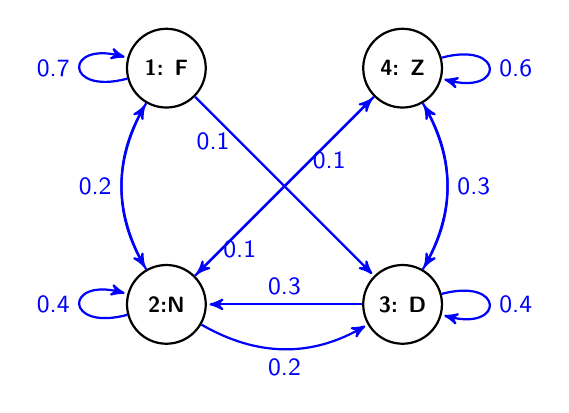
\begin{tikzpicture}[->,>=stealth',shorten >=1pt,auto,node distance=3cm,
                    thick,main node/.style={circle,draw,minimum size=1.cm,font=\sffamily\footnotesize\bfseries}]
%%%%%
\node[main node] (1)   {1: F};
  \node[main node] (2) [below of =1] {2:N};
 \node[main node] (3) [ right of=2] {3: D};
  \node[main node] (4) [right of=1] {4: Z};
  %%%%%%%
  \path[every node/.style={font=\sffamily\small, color=blue}, blue]
    (1)  %%%%%%%%%%%%%
        edge [loop left] node {0.7} (1)
        edge [bend right] node[left] {0.2} (2)
     edge [near start] node[left] {0.1} (3)
    (2) %%%%%%%%%%%%%
        edge [loop left] node {0.4} (2)
        edge [bend left] node[below] {} (1)
        edge [bend right] node[below] {0.2} (3)
         edge [near start] node[below] {0.1} (4)
    (3) %%%%%%%%%%%%%
        edge [loop right] node {0.4} (3)
       edge [bend right] node[right] {0.3} (4)
       edge [] node[above] {0.3} (2)
      (4) %%%%%%%%%%%%%
       edge [loop right] node {0.6} (4)
            edge [bend left] node[left] {} (3)
                 edge [below] node[near start] {0.1} (2);
\end{tikzpicture}
\end{center}
}
%\vs{.5}
\tasksAS{2}{2}{
\task What is the probability that a student who is currently in the Flow state will be in the Zoning Out state 2 minutes later?\\
\sol{
\large{	
\al{ S&=
 \begin{blockarray}{cc}
 \begin{block}{c[c]}
\fs{1} & 1 \\
 \fs{2} & 0 \\
 \fs{3}& 0\\
\fs{4} & 0 \\
 \end{block}
 \end{blockarray}\\
S_2&=P^2\cdot S
= \begin{blockarray}{cc}
 \begin{block}{c[c]}
\fs{1} & 0.53 \\
 \fs{2} & 0.25 \\
 \fs{3}& 0.17\\
\fs{4} & 0.05 \\
 \end{block}
 \end{blockarray}
}
The student has a $53\%$ probability to still be in a Flow state.
}
}
\task If a student starts class in Flow mode, what is the probability that they are still in a Flow state at the end of a $75$ minute class? In a Neutral state? A Distracted State? Zoned Out?
\sol{
\large{	
\al{ S&=
 \begin{blockarray}{cc}
 \begin{block}{c[c]}
\fs{1} & 1 \\
 \fs{2} & 0 \\
 \fs{3}& 0\\
\fs{4} & 0 \\
 \end{block}
 \end{blockarray}\\
S_{75}&=P^{75}\cdot S
= \begin{blockarray}{cc}
 \begin{block}{c[c]}
\fs{1} & 0.167598 \\
 \fs{2} & 0.251397 \\
 \fs{3}& 0.296089\\
\fs{4} & 0.284916 \\
 \end{block}
 \end{blockarray}
}
\itemI{
\item  Flow: $\approx 16.8\%$ .
\item  Neutral: $\approx 25.1\%$ 
\item  Distracted: $\approx 29.6\%$ 
\item  Zoned Out: $\approx 28.5\%$
}
}
}
%\task  Does this model predict that starting in a different state besides Flow will result in different probabilities for ending class in Flow or Zoned Out state?
\newpage
\task* In this model, students who are in Flow state or Neutral state are considered to be {\em engaged}. Students in a Distracted or Zoned Out state are considered to be {\em unengaged}.  For each possible starting state, determine the probability that students will be engaged by the end of class. \\

\sol{
For each of the $4$ possible starting states, 
\al{ S&=
 \begin{blockarray}{cc}
 \begin{block}{c[c]}
\fs{1} & 1 \\
 \fs{2} & 0 \\
 \fs{3}& 0\\
\fs{4} & 0 \\
 \end{block}
 \end{blockarray}
 , S=
 \begin{blockarray}{cc}
 \begin{block}{c[c]}
\fs{1} & 0 \\
 \fs{2} & 1 \\
 \fs{3}& 0\\
\fs{4} & 0 \\
 \end{block}
 \end{blockarray}
 , S=
 \begin{blockarray}{cc}
 \begin{block}{c[c]}
\fs{1} & 0\\
 \fs{2} & 0 \\
 \fs{3}& 1\\
\fs{4} & 0 \\
 \end{block}
 \end{blockarray}
  , S=
 \begin{blockarray}{cc}
 \begin{block}{c[c]}
\fs{1} & 0\\
 \fs{2} & 0 \\
 \fs{3}& 0\\
\fs{4} & 1 \\
 \end{block}
 \end{blockarray}
 \\
S_{75}&=P^{75}\cdot S
= \begin{blockarray}{cc}
 \begin{block}{c[c]}
\fs{1} & 0.167598 \\
 \fs{2} & 0.251397 \\
 \fs{3}& 0.296089\\
\fs{4} & 0.284916 \\
 \end{block}
 \end{blockarray}
 }
All long term outcomes are the same and do not depend on starting state. In particular, $$\limn S_n= \begin{blockarray}{cc}
 \begin{block}{c[c]}
\fs{1} & 0.167598 \\
 \fs{2} & 0.251397 \\
 \fs{3}& 0.296089\\
\fs{4} & 0.284916 \\
 \end{block}
 \end{blockarray}$$
The probability students will be  engaged at the end of class is:
$$ 0.167598+ 0.251397 \approx 41.9\%$$ 
and thus the probability students will be unengaged is $ 1-.419=58.1\%$

}
\vs{2}
\task* If the student decides to put their phone away for the entire class and thus reduces $P_{3,3}$ from $0.4$ to $0.2$, how does this impact their engagement at the end of class? Note that you will have to make some assumptions about the probability to move from Distracted to Zoned Out and the probability to move from Distracted to Neutral. Explain your assumptions and the impact on engagement at the end of class.
\sol{
The total probability for each column must add to $1$.  Thus we must compensate for reducing $P_{3,3}$ from $0.4$ to $0.2$ by increasing other probabilities associated with the Distracted state.
\\\\
 One such assumption could be that the student benefits from putting their phone away and thus increases probability to move from Distracted to Neutral. This changes $P_{3,2}$ from $0.3$ to $0.5$. The resulting transition matrix from these two changes is  
 \large{	
$$P=
 \begin{blockarray}{ccccc}
&\fs{1}& \fs{2} &\fs{3} &\fs{4}   \\
 \begin{block}{c[cccc]}
\fs{1} & 0.7& 0.2 & 0 &0 \\
 \fs{2} & 0.2&0.4 &0.5&0.1 \\
 \fs{3}& 0.1&0.3&0.2&0.3\\
\fs{4} & 0& 0.1 & 0.3 &0.6 \\
 \end{block}
 \end{blockarray}
$$
}


For each of the $4$ possible starting states, 
\al{ S&=
 \begin{blockarray}{cc}
 \begin{block}{c[c]}
\fs{1} & 1 \\
 \fs{2} & 0 \\
 \fs{3}& 0\\
\fs{4} & 0 \\
 \end{block}
 \end{blockarray}
 , S=
 \begin{blockarray}{cc}
 \begin{block}{c[c]}
\fs{1} & 0 \\
 \fs{2} & 1 \\
 \fs{3}& 0\\
\fs{4} & 0 \\
 \end{block}
 \end{blockarray}
 , S=
 \begin{blockarray}{cc}
 \begin{block}{c[c]}
\fs{1} & 0\\
 \fs{2} & 0 \\
 \fs{3}& 1\\
\fs{4} & 0 \\
 \end{block}
 \end{blockarray}
  , S=
 \begin{blockarray}{cc}
 \begin{block}{c[c]}
\fs{1} & 0\\
 \fs{2} & 0 \\
 \fs{3}& 0\\
\fs{4} & 1 \\
 \end{block}
 \end{blockarray}
 \\
S_{75}&=P^{75}\cdot S
= \begin{blockarray}{cc}
 \begin{block}{c[c]}
\fs{1} & 0.204444 \\
 \fs{2} & 0.306667 \\
 \fs{3}& 0.235556\\
\fs{4} & 0.253333 \\
 \end{block}
 \end{blockarray}
 }

The decision to put away the phone increases the probability that students will be engaged at the end of class to $$0.204444+0.306667\approx 51.1\%$$

}
%\vs{2} 
\task* What might account for the fact that the transition probability from Zoned Out to Flow state  (i.e. $P_{1,4}$) equal to $0$ in this model? 
\sol{
There are many reasonable answers.  Here is one.\\\\
{\em 
 This probability mimics realistic behavior. We don't go from being completely disengaged to highly focused in an instant. Being highly focused requires effort to understand what is most important in the moment an thus to ignore that which is less important. This requires a process that does not occur in an instant.
 }

}
}
}
}
\newpage




\end{document}  
